\chapter{Methodology}
\label{sec:methodology}

As this thesis's endeavor was to merge and enhance various aspects of the LORNA project, the complexity lay rather in understanding the existing work and its interfaces as opposed to the challenging methodology pursued in the novel contributions. Therefore, the implementation aspect of this work carries more weight than the theoretical decision-making associated with it.

The autonomy framework\citep{Autonomy} allows us to fly independent missions at cruise altitudes of 100+ m. The structure from motion approach captures 3D information during traversal as its adaptive baseline allows it to perceive high-quality depth information at such high altitudes. This information can be used by LSD to detect landing sites during missions. 

At low altitudes, SFM works as well, but surrounded by obstacles, the need for lateral motion poses significant risk. A local state estimator is, by nature, prone to accumulating an estimation error, and the same holds for the structure from motion algorithm. Our terrain knowledge can thus become void. 

To overcome this issue, a range sensor can be used. An obvious consideration is LiDAR. However, a LiDAR sensor produces rather sparse point clouds unless a newer sensor, like Ouster's OS1-128\footnote[1]{https://ouster.com/products/hardware/os1-lidar-sensor} sensor, is used. In that case, there remains the weight issue with the sensor's 495g. As the drone is going to fly in Mar's very thin atmosphere, this isn't feasible. 

Staying with the project's theme of visual sensors, a stereo camera poses a solution as it offers in-place triangulation with a very low weight ($\approx 10g$). Therefore, in this thesis, I present a stereo camera range node implementation to remedy the shortcomings at low altitudes.


\section{Stereo Camera}\label{sec:stereo_methodology}

The implementation of the stereo camera sensor itself is very straightforward as simply duplicating an existing camera, offsetting it an adequate distance to resemble the real model, and setting the parameters to equal the hardware, results in the desired outcome.

The simulated camera sensors used for this had the following properties:

\begin{itemize}
    \item Image width: 640 pixels
    \item Image height: 480 pixels
    \item fx: 275.42px
    \item fy: 276.27px
    \item cx: 342.22
    \item cy: 234.66
\end{itemize}

The input to the stereo camera depth node is the two camera images and the drone's base link pose. Processing this information is different from the existing SFM algorithm, so a new depth generation node was implemented. 

As mentioned in \cref{sec:relwork}, state-of-the-art deep learning-based stereo depth methods have considerably higher computational overhead. Due to the embedded CPU's computation limitations, this restricts us to using classical algorithms such as OpenCV's widely used implementations of Heiko Hirschmüller's approach (\citep{Stereo}).

The initial goal of the stereo camera implementation of this work was to show proof of concept for this approach of depth detection without lateral motion. Due to personal experience with the OpenCV library, the initial choice of stereo depth method was OpenCV's StereoSGBM algorithm. This algorithm is introduced in \cref{subsec:disparity_creation}.

JPL has its own visual library, JPLV, containing a stereo-matching method already in use for SFM, that will likely be a better choice for the future of the stereo depth node as well. This is because of three reasons:
\begin{itemize}
    \item JPLV has a faster implementation which is beneficial for Mars missions flown with a limited processor.
    \item JPLV supports the CAHVORE camera model JPL uses for its visual applications. OpenCV, however, does not.
    \item Lastly, JPLV was created and is maintained in-house, which is always preferable to open source solutions. 
\end{itemize}
However, for the proof of concept of the contributions in this work, especially using camera images without distortion, there was no specific reason to switch away from the preliminary StereoSGBM implementation. Therefore, the continuation thereof was pursued.

\subsection{Stereo Camera Advantages}

The specific advantage of a stereo camera implementation when compared to SFM can be summarized in the following points:

\begin{itemize}
    \item No necessity of lateral motion
    \item Hardware depth perception
    \item DEM conversion
    \item Efficiency
\end{itemize}

\subsubsection{Lateral Motion}

As already mentioned above, lateral motion is an undesirable necessity for a rotorcraft in unknown terrain. 

In this setup, the structure from motion approach is based on a keyframe buffer, which needs to be filled with image-pose pairs at different horizontal positions in order to start acquiring depth information. The current setting in the implementation \citet{SFM} uses 6 keyframes. Therefore, for a single point cloud, it is necessary to move laterally 6 times to start perceiving depth. With a necessary baseline of 0.23\footnote[2]{Calculated by using the formula introduced in \cref{eq:depth_error_formula} at 2.5 m altitude, a focal length of 275.42, a subpixel disparity error of 0.5 and an acceptable depth error of 10 cm} m, that would be over a meter before SFM start collecting data. Note that, As described in \cref{subsubsec:setup:aggregation}, LSD needs to converge for some time before high quality landing sites can be detected. Therefore, even more terrain would need to be traversed. We would like to avoid this necessity when flying the rotorcraft at such low altitudes.

\subsubsection{Software vs Hardware Depth Perception}

Structure from Motion, a software node that relies on camera poses supplied by a state estimator, is, by design, subject to inaccuracies. A depth node based on a stereo camera, on the other hand, works with a fixed, rigid baseline between the camera views. Thus, for low-altitude flights that bear the danger of collision, a more robust hardware approach is preferred.

\subsubsection{DEM Conversion}

At low altitudes the image footprint of the tracking camera is only a few meters in each dimension. Therefore, to repeatedly observe the same terrain and let the measurements converge, the drone, using SFM,  would have to fly forth and back over the same area. With a stereo camera implementation the drone can simply hover above the potential sites to gather this information.

\subsubsection{Efficiency}

All in all, the SFM setup allows us to detect a landing site at course altitude and after traversing horizontally to that location, we can simply descend to a stereo camera friendly altitude to hover for the verification. Therefore, simply descending to a low altitude and hovering for a short duration is significantly more efficient than flying lateral patterns at different altitudes above a landing site.

\section{Ground Truth Depth}

For evaluating the stereo depth node as well as proof of concept aspirations of the autonomous landing behavior introduced hereafter, a ground truth is required. 

Additionally, GT was important because, at the time of this work, the structure from the motion node showed frequent signs of unreliability. See \cref{subsec:sfm_insufficiencies} for the evaluation thereof.

\subsection{Ground Truth Implementation}
The simulation already supplied the ground truth pose of the drone's base link through the ROS bridges. When applying the static camera transform to it, this yielded the ground truth camera pose. Using Gazebo's depth camera sensor\footnote[3]{As there was a bug in Gazebo's source code, the depth camera couldn't be used out of the box. More on this in \cref{sec:appendix:gz_depth_camera}.}, a ground truth point cloud could be created.

The depth camera creates the image using traced rays, which fill a pixel with the centermost range value that a ray detected.

Looking at \cref{fig:gt_lsd_debug}, we can see that the ground truth point clouds yield very clean and easily interpretable LSD DEMs. \cref{fig:gt_lsd_debug_reference} shows the reference view of the terrain in the Gazebo simulation.

\begin{figure}[h]
\centering
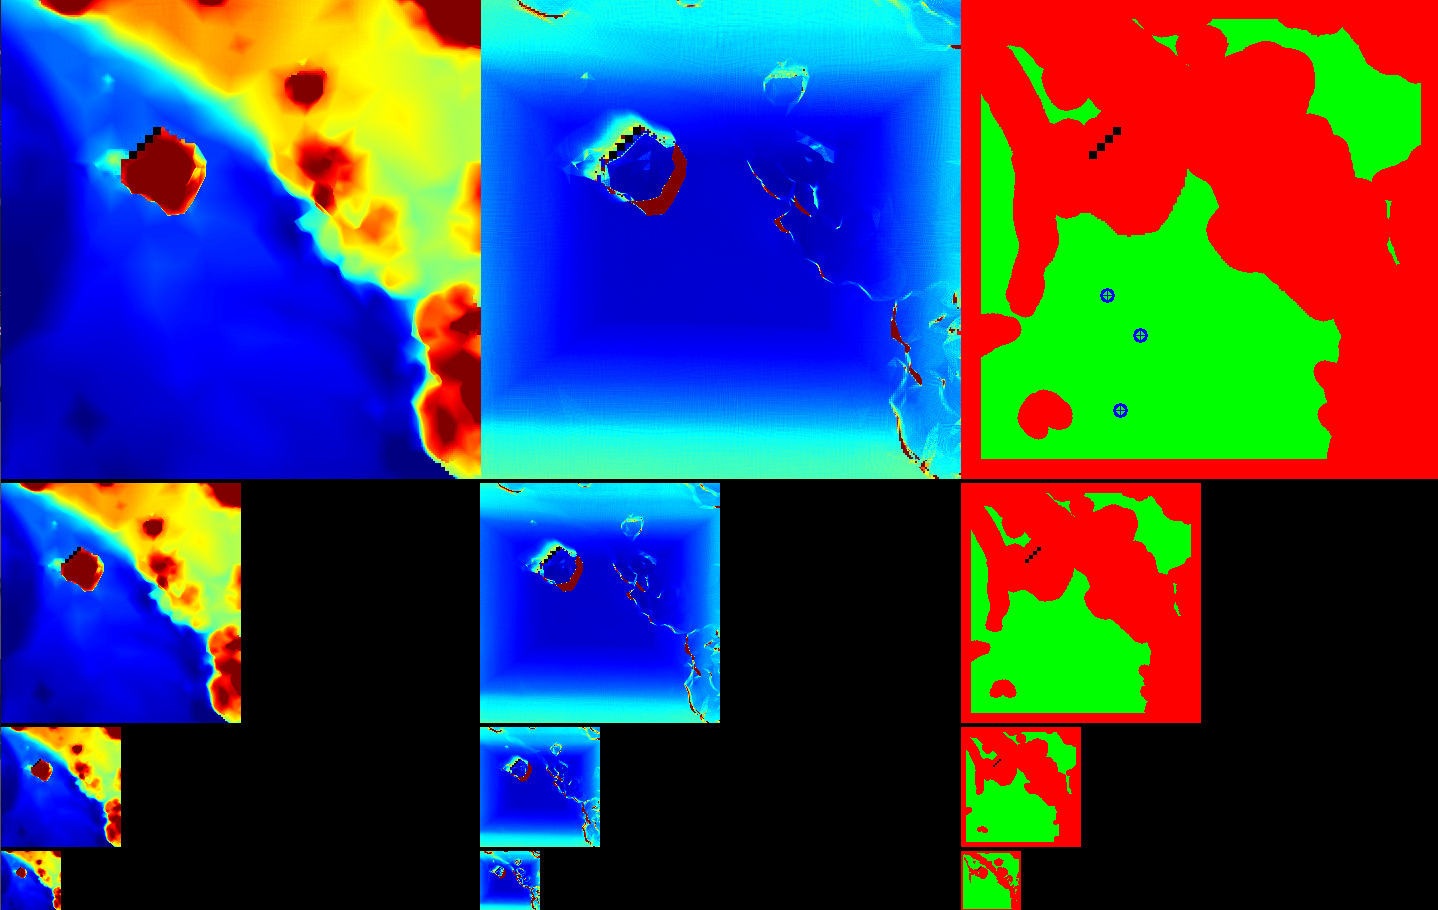
\includegraphics[scale=0.25]{images/methodology/lsd_debug_image.png}
\caption{LSD debug image using a GT point cloud}
\label{fig:gt_lsd_debug}
\end{figure}

\begin{figure}[h]
\centering
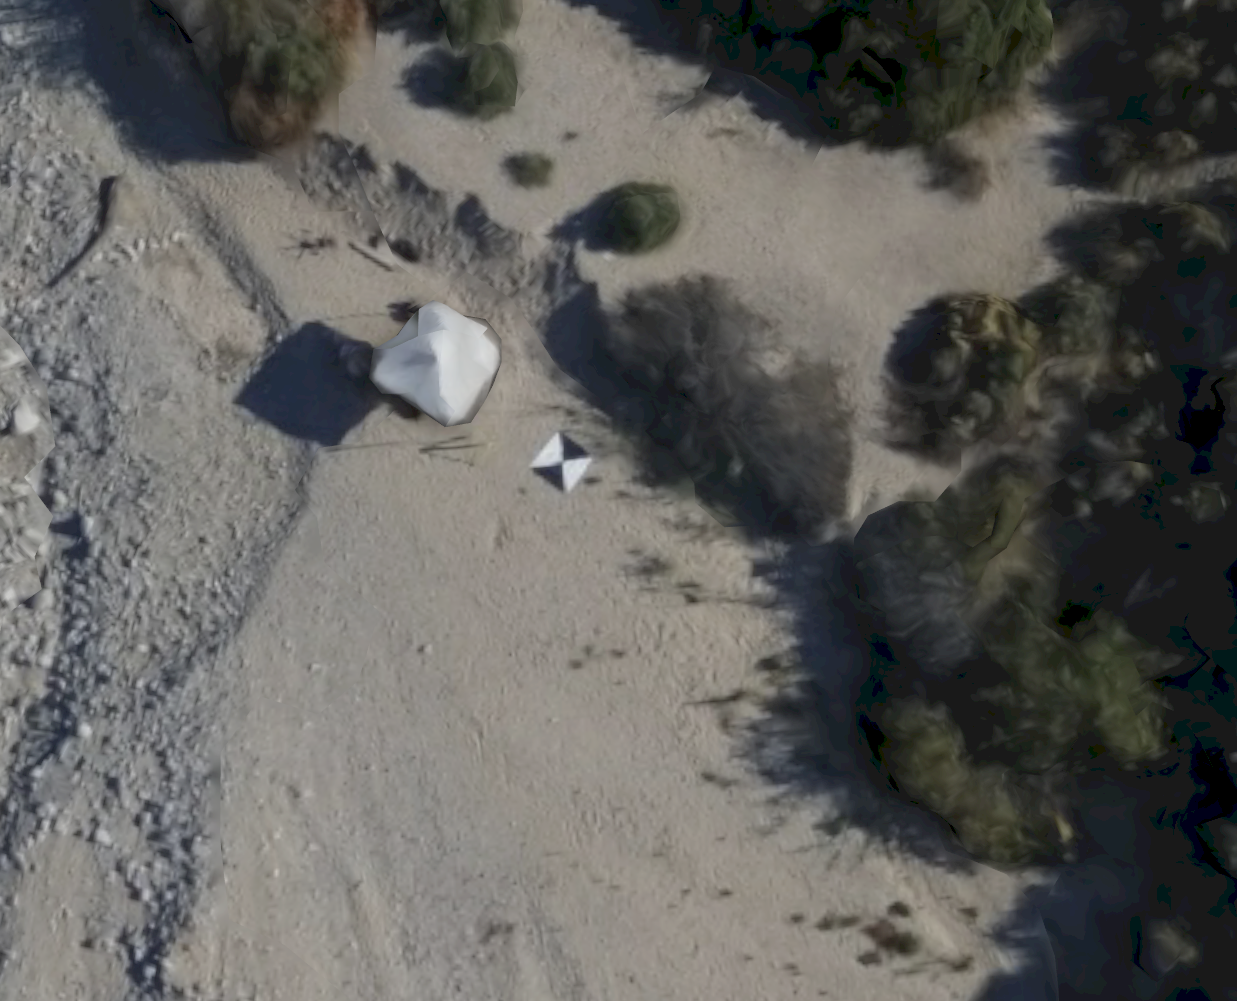
\includegraphics[scale=0.25]{images/methodology/lsd_debug_reference.png}
\caption{LSD debug image simulation terrain reference}
\label{fig:gt_lsd_debug_reference}
\end{figure}
\clearpage %HERE

\subsection{Comparability to SFM}

This is sufficient for a qualitative analysis of the stereo-depth node. However, to use the ground truth as an alternative for SFM, one must ensure that the GT quality is not too good. For instance, SFM, like the stereo camera depth, has a depth error associated with its point cloud creation. At high altitudes, this can lead to the neglect of small (but mission-threatening) rocks. So, in order to test the autonomous landing pipeline with ground truth, I had to make sure that small rocks of about 10 cm in diameter were not seen by the GT at a cruise altitude of 100 m.

For this, the test setup shown in \cref{fig:gt_test_setup1} and \cref{fig:gt_test_setup2} was used.

On the Arroyo map, three cylinders of different sizes were placed. On each cylinder a small rock of 10 cm diameter was placed. The drone was then flown over the test setup at an altitude up to 100 m to detect the scene once with SFM and once using the GT depth. The goal was to find out, whether the ground truth depth quality would have to be artificially decreased, using Gaussian or median filtering for instance, in order to make it more comparable to SFM.
\clearpage %HERE

\begin{figure}[ht]
\centering
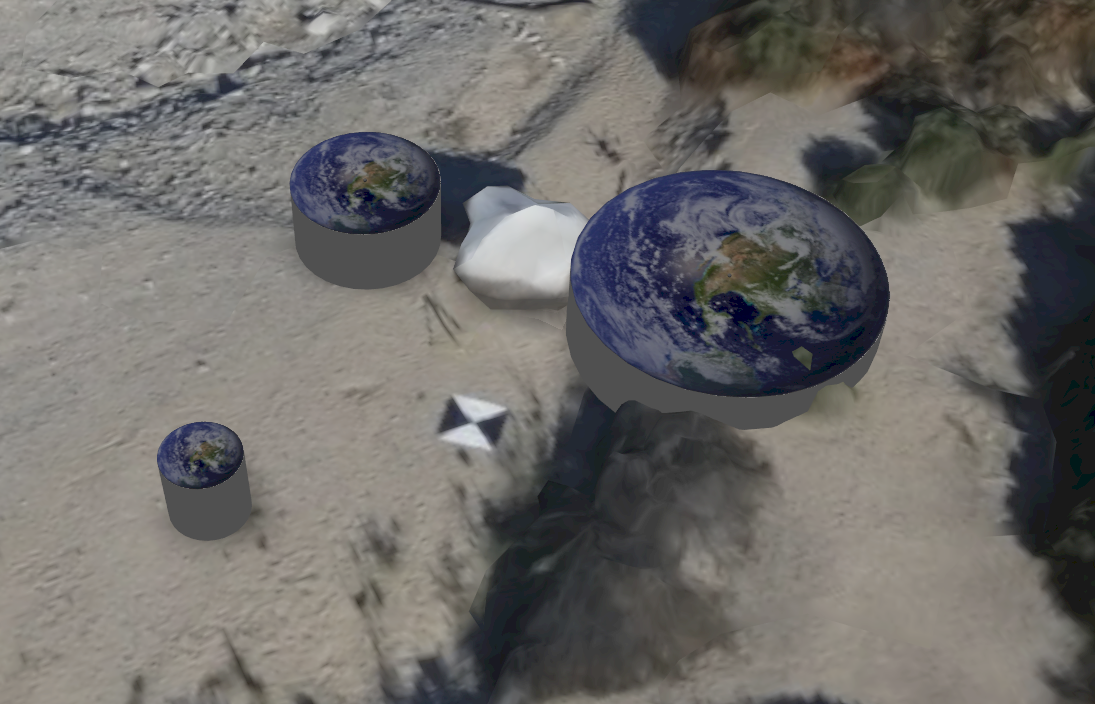
\includegraphics[scale=0.3]{images/methodology/test_setup1.png}
\caption{GT test setup1: Three cylinders of different sizes (4, 2, and 1 m diameter) were placed on the map}
\label{fig:gt_test_setup1}
\end{figure}

\begin{figure}[ht]
\centering
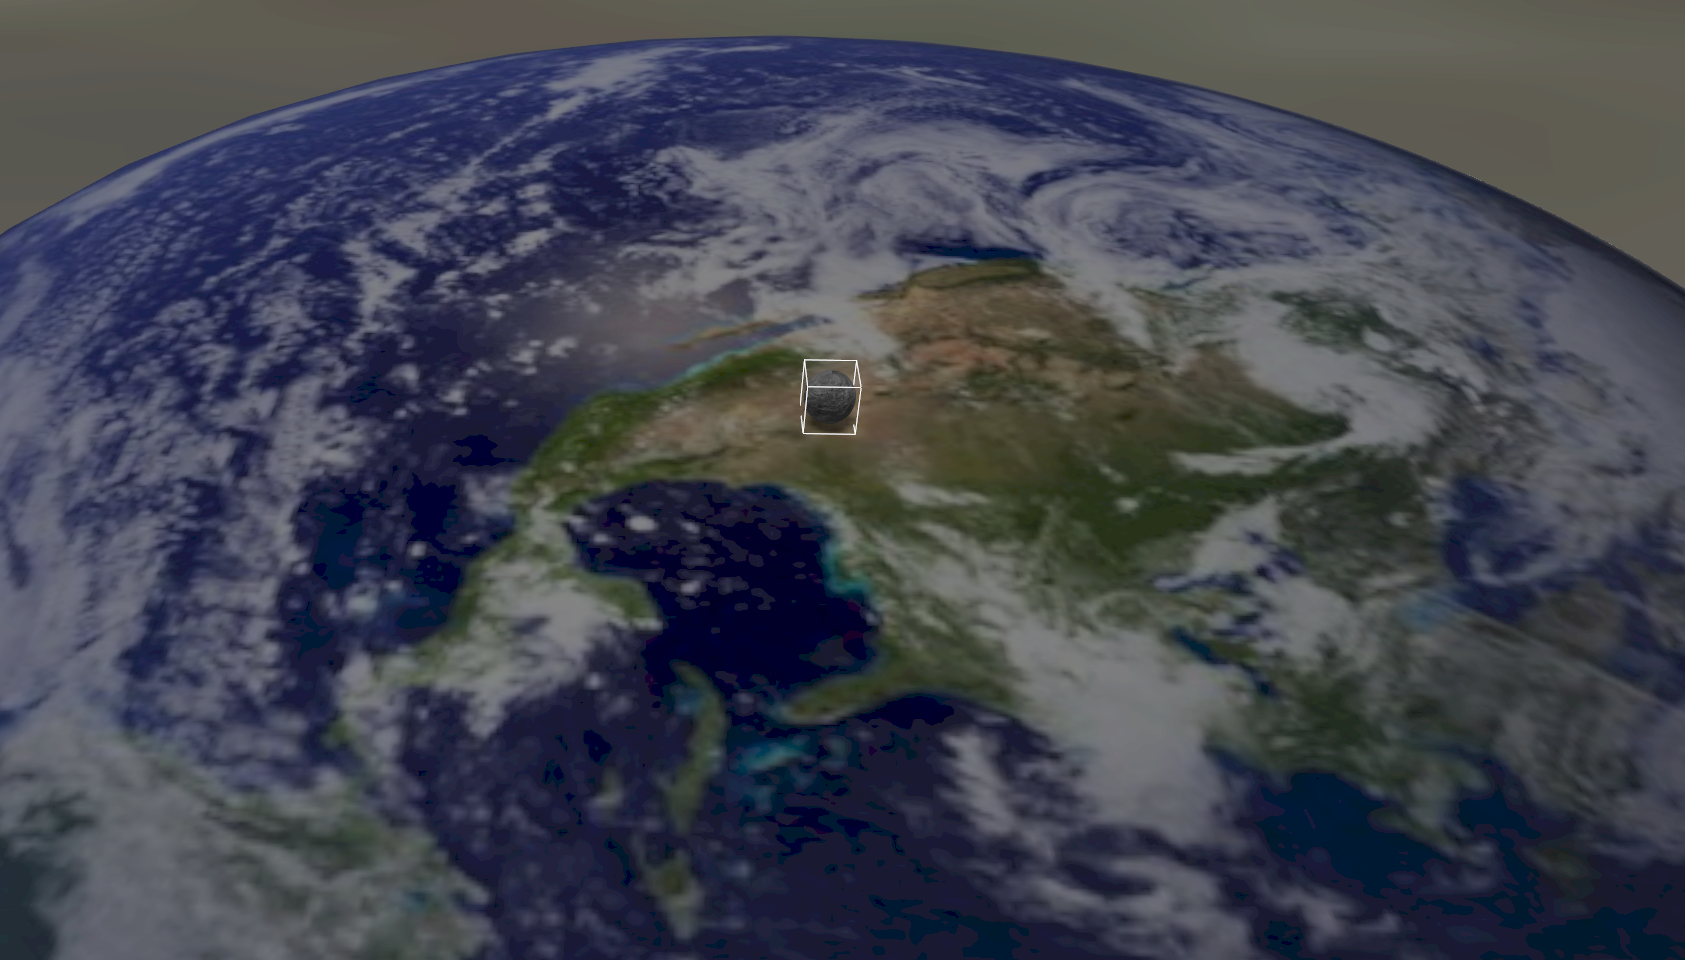
\includegraphics[scale=0.195]{images/methodology/test_setup2.png}
\caption{In the middle of each cylinder, a rock of 10 cm diameter was placed}
\label{fig:gt_test_setup2}
\end{figure}

\clearpage %HERE

Looking at \cref{fig:gt_test_gt} and \cref{fig:gt_test_sfm}, one can see that, though the SFM quality is visibly worse, neither SFM nor GT detected the small rocks on the platforms. This can be seen because in both Debug images, the center of the platforms was considered a landing site even though there was the rock, which should definitely prevent the detection of a valid landing site in the very center.

Therefore, the ground truth depth could be used to test the autonomous landing pipeline without making a landing site verification step at low altitudes redundant.

\begin{figure}[ht]
\centering
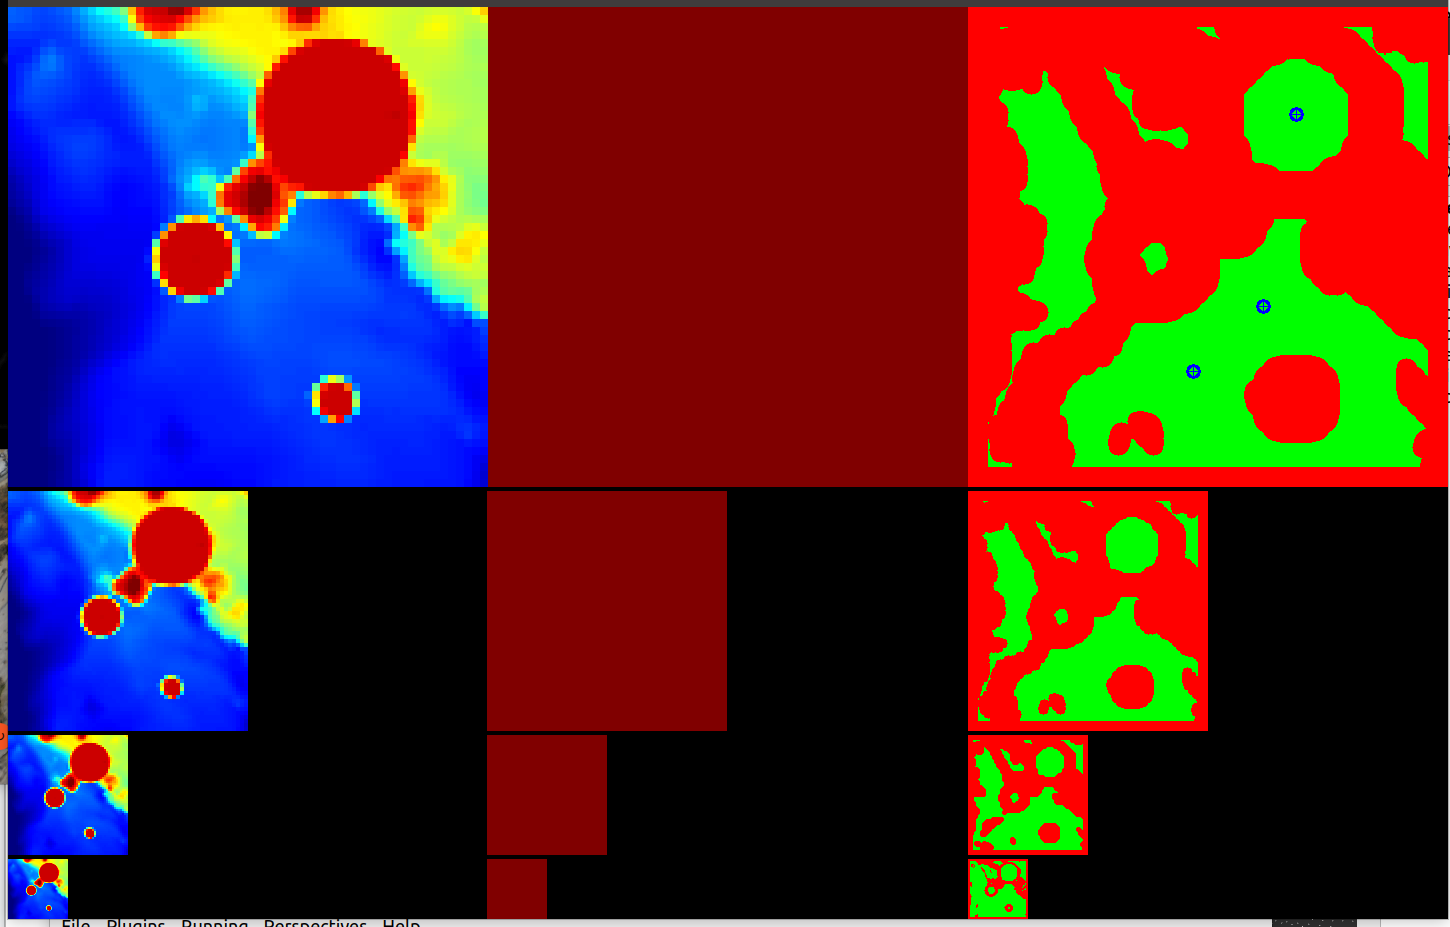
\includegraphics[scale=0.22]{images/methodology/GT.png}
\caption{Ground truth result of the GT test}
\label{fig:gt_test_gt} 
\end{figure}

\begin{figure}[ht]
\centering
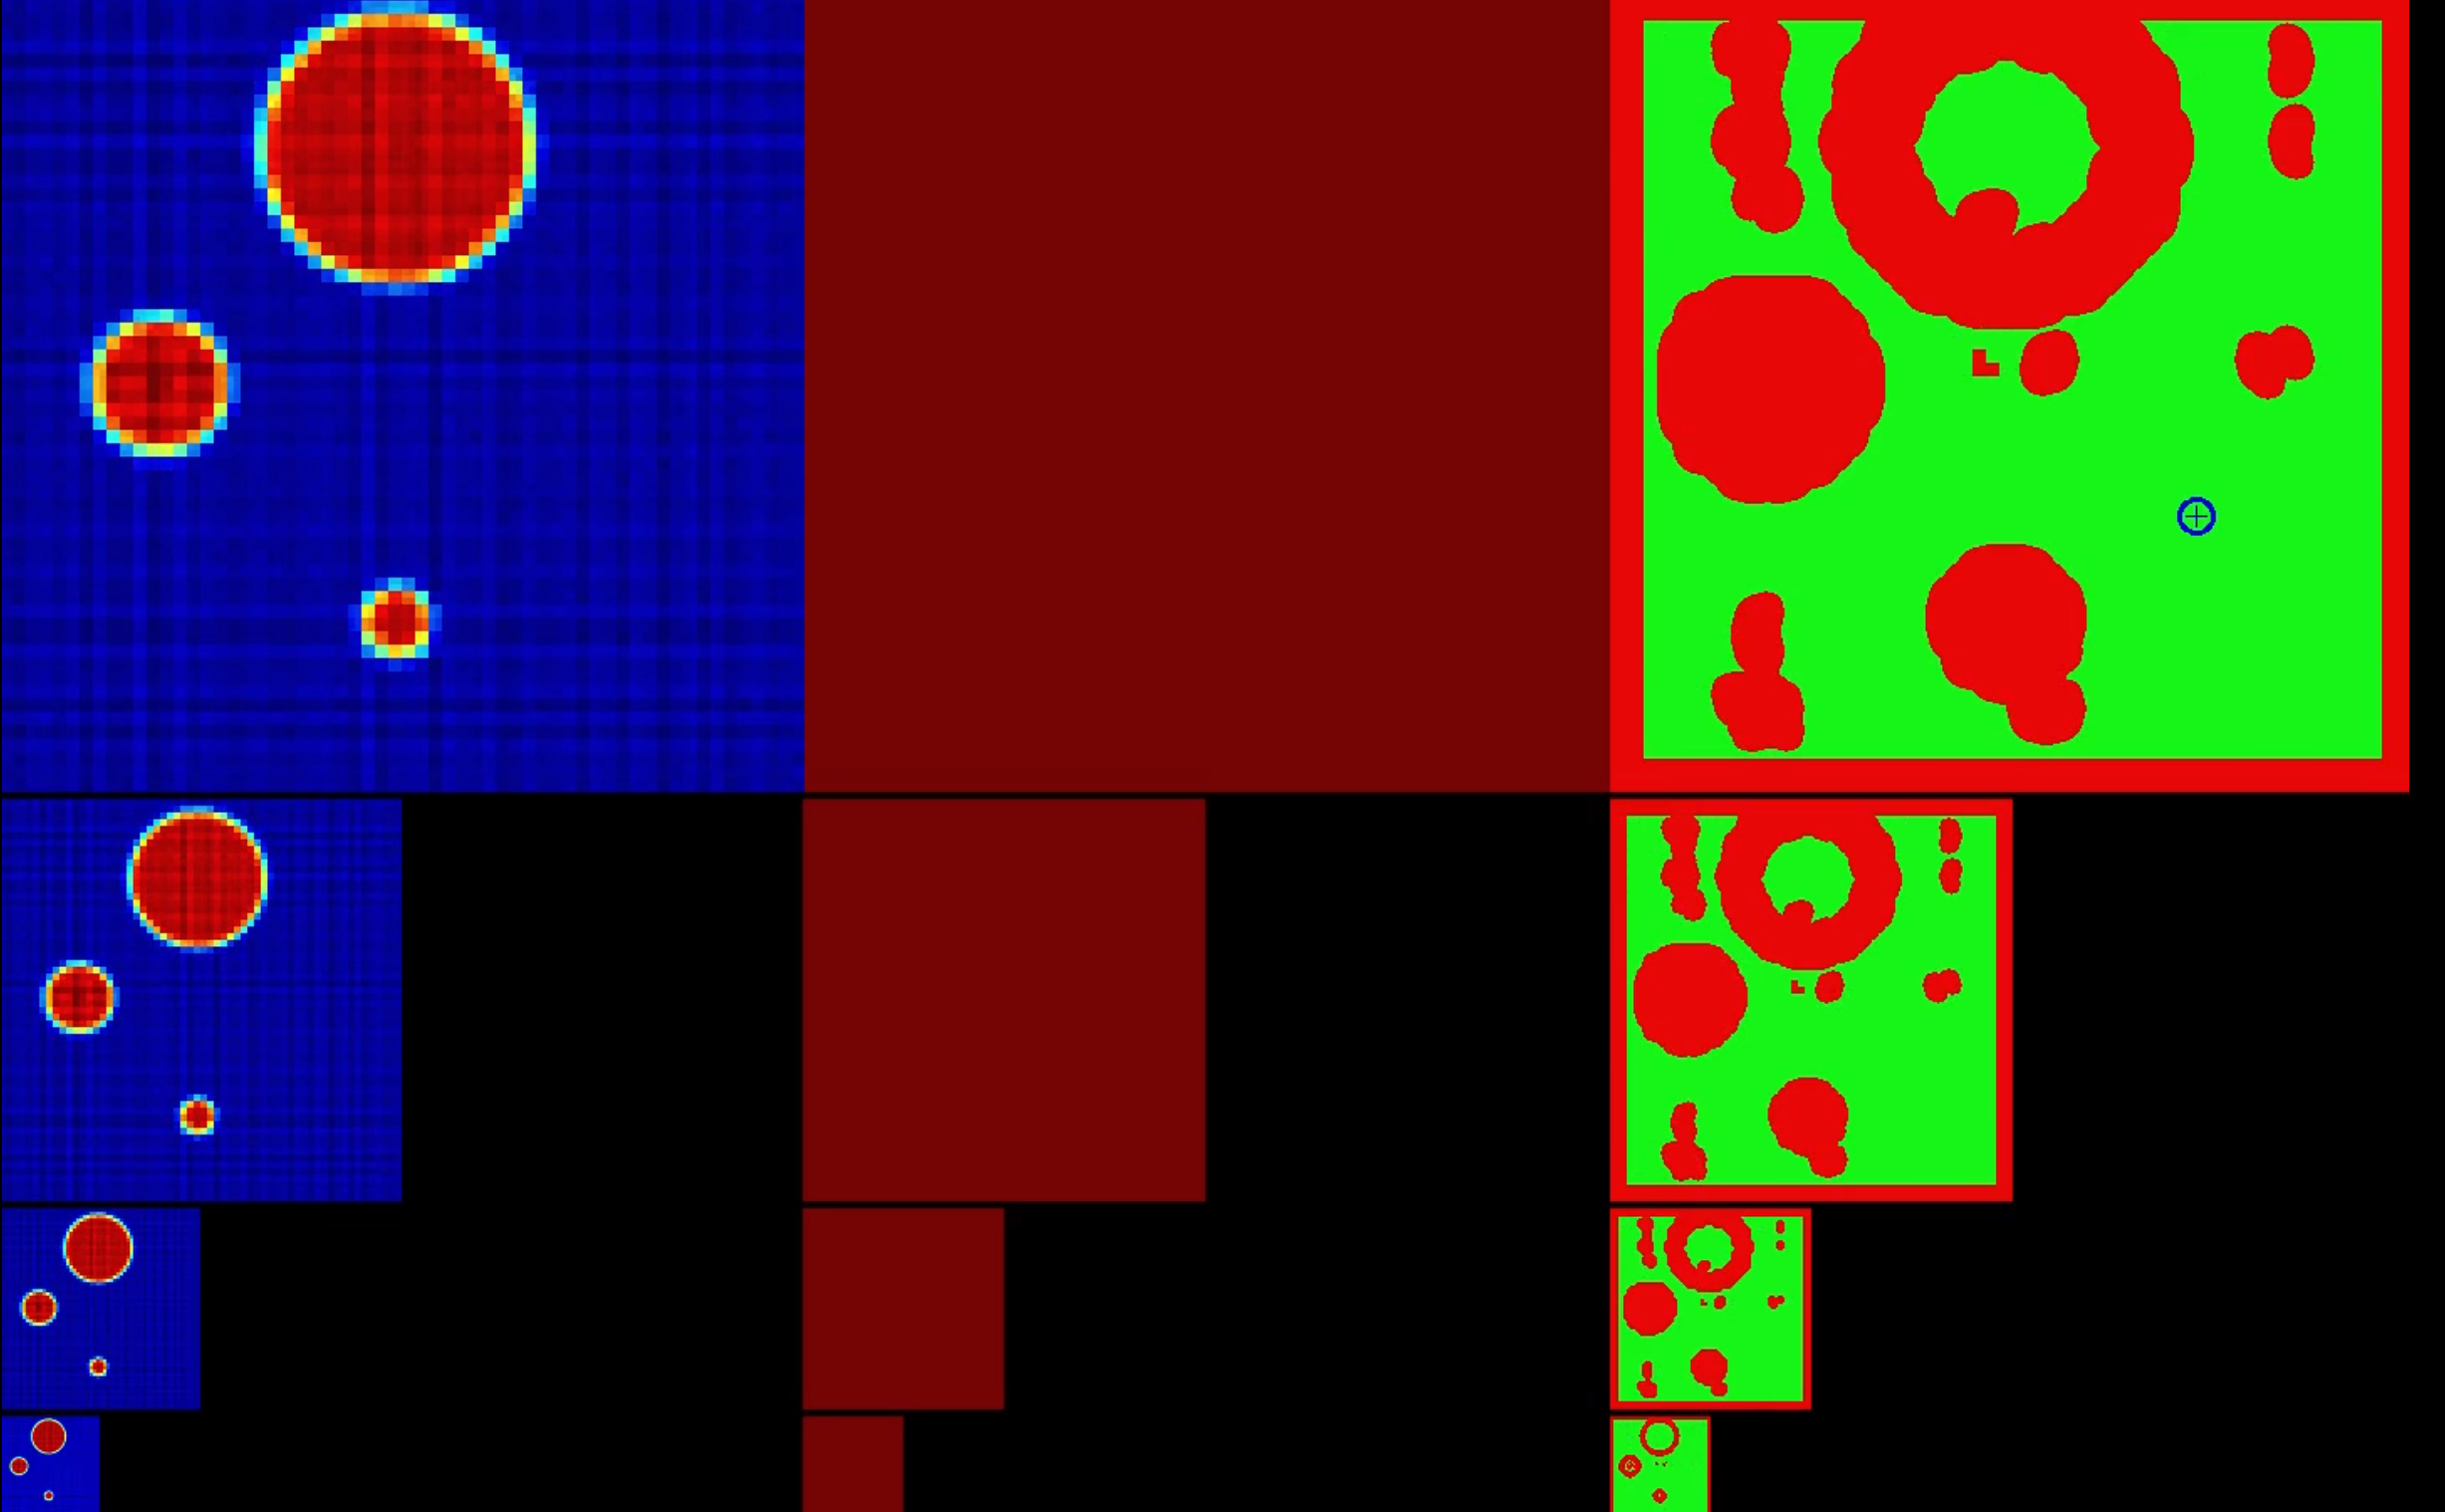
\includegraphics[scale=0.22]{images/methodology/SFM.png}
\caption{SFM result of the GT test}
\label{fig:gt_test_sfm}
\end{figure} 



\clearpage %HERE
\section{Autonomous Landing Procedure}

After implementing a stereo camera as a low-altitude alternative to SFM and ensuring a correct ground truth comparison, the main contribution of this work could be tackled: bringing the visual landing site pipeline together with the autonomy framework to achieve reliable autonomous landing in unknown terrain.

The manner of implementation for the autonomous landing sequence was more or less given by the system architectures that this work combines. The two crucial points of the methodology were the interface between the autonomy framework and the landing site detector and the implementation of the decision-making in the behavior tree of the landing node as well as the landing site manager.

\subsection{LSD - Autonomy Interface}

Both the autonomy and the landing site detection node had to be altered for the interface with autonomy.

\begin{itemize}
    \item Landing site detection output

    Prior to this work, LSD only published the location of one landing site. To give the autonomy more information to make adequate decisions and to avoid stagnation on a single overconfident landing site, LSD was changed to first publish three landing sites each iteration and secondly yield additional characteristics with each output landing site.
    \item Landing site interface of the autonomy

    The autonomy framework was changed to correctly receive and handle the incoming landing sites with all the newly associated properties. Furthermore, novel landing site handling concepts like re-detection and banishment were introduced.    
\end{itemize}

\subsection{Autonomous Landing Behavior}

As previously explained, the landing behavior in the autonomy framework is implemented using a behavior tree consisting of small modular and expandable actions. The existing BT framework and the available actions prior to this work are shown in \cref{subsec:setup:behavior_tree}.

The two paramount qualities in pursuit of which the landing behavior was designed are safety and efficiency. Naturally, safety is the first-most concern. We want a reliable autonomous landing procedure for the drone to repeatedly land safely. However, the more efficient it is, the more daring science missions can be designed and the faster the red planet can be explored in detail.

For the conceptual design of the autonomous landing behavior, a fail-safe dogma was adopted, meaning that the drone never moved both horizontally and vertically. Instead, any required traversal was preceded by an adequate ascent to a safe height and followed by a vertical descent to the desired altitude at the new location. Secondly, the available landing site characteristics were used to enhance the overall efficiency. 

